\chapter[Integración de variable real]{Integración de funciones en $\mathbb{R}$}

En este breve capítulo veremos cómo es posible utilizar el teorema de los residuos y las formas de resolución de integrales de variable compleja para resolver integrales de variable real.

En el estudio de la integración compleja, como vimos en el capítulo \ref{chpt:integlacion_compleja}, es habitual interpretar una integral de línea como la integral de una función compleja sobre una curva parametrizada. La parametrización permite traducir la información geométrica de la curva en una integral ordinaria sobre un intervalo real. Este procedimiento es fundamental: toda integral de línea se reduce, en última instancia, a una integral real mediante una elección adecuada de parámetro.

Cuando el objetivo es evaluar integrales reales mediante técnicas de análisis complejo, el razonamiento se invierte. Se observa la integral real dada y se la interpreta como la parte real (o imaginaria, según el caso) de la integral de una función compleja sobre cierta curva en el plano complejo. A partir de esa reinterpretación geométrica, la integral se completa en un contorno cerrado apropiado y se aplica el Teorema de los Residuos.

En síntesis, el método consiste en reconocer que una integral real puede verse como un caso particular de una integral de línea compleja cuya parametrización ya está implícita. Al ``deshacer'' esa parametrización y situarla en un contorno adecuado, la teoría de los residuos proporciona una herramienta poderosa para su evaluación. Esta perspectiva unifica ambos tipos de integrales y muestra cómo la geometría del plano complejo enriquece el análisis de integrales reales.

\section{Integrales trigonométricas}
\label{sec:integrales_reales_trigonometricas}

Primero se consideran integrales del tipo 
\begin{equation}
  I = \int_0^{2\pi} K(\cos(\theta),\sin(\theta))d\theta
\end{equation}
en donde $K$ es una función racional de $\cos(\theta)$ y $\sin(\theta)$, por ejemplo 
$$
F(\cos(\theta),\sin(\theta))=f(\theta)=\frac{\sin^2\theta}{5-4\cos\theta}
$$
y es finita sobre el intervalo de integración, es decir $F$ no tiene comportamiento asintótico en el intervalo.

La idea será probar que esta integral real es igual a una integral de cierta función compleja sobre el círculo unitario. Después usará el teorema del residuo para evaluar esta integral compleja, obteniendo el valor de la integral real.

Para llevar a cabo esta estrategia, sea $\gamma$ el círculo unitario, recorrido en sentido antihorario. Parametrizamos $\gamma$ por $\gamma(\theta)=e^{j\theta}$ para $0\leqslant \theta \leqslant 2\pi$. En esta curva $z=e^{j\theta}$ y $\bar{z}=e^{-j\theta}=1/z$, así
\begin{align*}
  \cos(\theta) =& \frac{1}{2}\left( e^{j\theta}+e^{-j\theta} \right) = \frac{1}{2}\left(z+\frac{1}{z}\right) \\ 
  \sin(\theta) =& \frac{1}{2j}\left( e^{j\theta}-e^{-j\theta} \right) = \frac{1}{2j}\left(z-\frac{1}{z}\right)
\end{align*}
Y, podemos obtener una expresión para $d\theta$ a partir de la definición de diferencial 
$$
dz=je^{j\theta}d\theta = jzd\theta \quad \Rightarrow \quad d\theta = \frac{1}{jz}dz
$$
Ahora se tiene 
$$
\oint_\gamma K\left(\frac{z+\bar{z}}{2},\frac{z-\bar{z}}{2j}\right)\frac{1}{jz}dz = \int_0^{2\pi}K(\cos(\theta),\sin(\theta))d\theta
$$
Esto convierte la integral a evaluar en la integral de la función compleja $f(z)$ sobre el círculo unitario, donde 
$$
f(z)=K\left(\frac{z+\bar{z}}{2},\frac{z-\bar{z}}{2j}\right)\frac{1}{jz}
$$
Entonces, para resolver la integral real, se usa el teorema del residuo para evaluar $\oint_\gamma f(z)dz$, obteniendo así,
\begin{equation}
  \boxed{\int_0^{2\pi}K(\cos(\theta),\sin(\theta))d\theta = j2\pi \sum_{k=1}^n \res_{z=z_k}f(z)}
\label{eq:integral_real_trig}
\end{equation}
La suma de la derecha es sobre todos los polos $z_1,z_2,\dots,z_n$ encerrados por el círculo unitario. La función $f$ debe ser analítica sobre la curva, por tanto no pueden haber singularidades en el círculo unitario mismo.

Así que el procedimiento para evaluar $\int_0^{2\pi} K(\cos\theta,\sin\theta)d\theta$ consiste en calcular $f(z)$, determinar sus polos dentro del círculo unitario, evaluar ahí los residuos y aplicar la ecuación \eqref{eq:integral_real_trig}.

\begin{example}
  Demostrar, aplicando el método de evaluación de integrales reales visto, que 
  $$
  \int_0^{2\pi}\frac{1}{\sqrt{2}-\cos(\theta)}d\theta = 2\pi
  $$
  Se usa $\cos(\theta)=\frac{1}{2}(z+\bar{z})$ y $d\theta = dz/jz$. Así la integral se vuelve 
  $$
  \oint_\gamma \frac{dz/jz}{\sqrt{2}-\frac{1}{2}\left(z+\frac{1}{z}\right)} = \oint_\gamma \frac{1}{-\frac{j}{2}(z^2-2\sqrt{2}z+1)} dz
  $$
  Aplicando la fórmula resolvente para encontrar las raíces del denominador
  $$
  -\frac{2}{j}\oint_\gamma \frac{1}{(z-\sqrt{2}-1)(z-\sqrt{2}+1)}
  $$
  Así, vemos que si $z$ toma el valor $z_1=\sqrt{2}+1$ está fuera de $\gamma$. Sin embargo, si toma $z_2=\sqrt{2}-1$ está dentro de $\gamma$, entonces el residuo es 
  $$
  \res_{z=z_2}f(z)=\lim_{z\to z_2} \frac{1}{1-z_1} = \frac{1}{z_2-z_1} = \frac{1}{\sqrt{2}-1-\sqrt{2}-1} = -\frac{1}{2}
  $$
  Reemplazando este resultado para resolver la integral, resulta 
  $$
  -\frac{2}{j}\oint_\gamma \frac{1}{(z-z_1)(z-z_2)} =-\frac{2}{j}j2\pi\left(-\frac{1}{2}\right) = 2\pi 
  $$
  y, consecuentemente
  $$
  \int_0^{2\pi}\frac{1}{\sqrt{2}-\cos(\theta)}d\theta = 2\pi
  $$
  lo que se quería demostrar.
\end{example}

Al aplicar este método, si se obtiene un número que no es real, hay que verificar los cálculos, ya que una integral real tiene un valor real.

\section{Lema de Jordan}

El lema de Jordan\footnote{Matemático francés: Marie Ennemond Camille Jordan.} nos permitirá demostrar que pueden resolverse otro tipo de integrales reales además del que ya vimos en la sección anterior.

Si una función $Q(z)$ satisface las siguientes condiciones:
\begin{enumerate}
  \item $Q(z)$ es analítica en todo el semiplano superior, excepto en un número finito de polos.
  \item $Q(z)$ tiende uniformemente a cero cuando $z\to\infty$, para $0<\text{arg}(z)<\pi$.
  \item $m$ es un número real positivo (o bien $m\in\mathbb{R}^+$).
\end{enumerate}
Entonces, se cumple que 
\begin{equation}
  \lim_{R\to\infty} \left( \int_\gamma Q(z)\,e^{jmz}\, dz \right) = 0
  \label{eq:lema_de_jordan}
\end{equation}
Donde $\gamma$ es una semicircunferencia de radio $R$ y centro en el origen, como se muestra en la figura \ref{fig:curva_de_jordan}.

\begin{figure}[ht]
  \centering
  \begin{tikzpicture}[>=stealth]
    \path (-2.5,0) -- (-2,0); % solo para terminar de centrar
    \draw[->,gray] (-2,0) -- (2,0) node[right] {\scriptsize$\Re(z)$};
    \draw[->,gray] (0,-0.2) -- (0,2) node[above] {\scriptsize$\Im(z)$};

    \begin{scope}[decoration={
        markings,
        mark=at position 0.1 with {\arrow{>} \node[above right] {$\gamma$};},
        mark=at position 0.5 with {\arrow{>}},
        mark=at position 0.9 with {\arrow{>}},
      }]
      \draw[red,very thick,postaction={decorate}] (1.7,0) arc (0:180:1.7);
    \end{scope}
    \node[below] at (1.7,0)  {\scriptsize$R$};
    \node[below] at (-1.7,0) {\scriptsize$-R$};

    \draw[->] (0,0) -- (60:1.7);
    \draw[fill] (60:1.7) circle (1pt) node[above] {\scriptsize\color{black}$z$};
    \draw (0.5,0) arc (0:60:0.5) node[below=1pt] {\scriptsize\color{black}$\theta$};
  \end{tikzpicture}
  \caption{}
  \label{fig:curva_de_jordan}
\end{figure}

Como se ve en la figura \ref{fig:curva_de_jordan}, la variable que se desplaza a lo largo de $\gamma$ es $z=Re^{j\theta}$, por esta razón, cuando se dice $\lvert z \rvert \to \infty$ equivale a decir $R\to\infty$, dado que el módulo de $z$ es $R$
$$
z=Re^{j\theta} \Rightarrow \lvert z \rvert = \lvert Re^{j\theta}\rvert = R.
$$

La expresión \eqref{eq:lema_de_jordan} es el lema de Jordan y su demostración es muy extensa y complicada por lo cual la omitimos. Solo usaremos este resultado para obtener un nuevo tipo de integrales reales que pueden ser resueltas a través de la integración compleja.

\section{Integrales impropias}

En este apartado consideraremos integrales reales del tipo 
$$
\int_{-\infty}^\infty f(x)dx
$$
Tal integral, para la que el intervalo de integración no es finito, se denomina integral impropia, y significa que 
$$
\int_{-\infty}^\infty f(x)dx = \lim_{a\to-\infty} \int_a^0 f(x)dx + \lim_{b\to\infty} \int_0^b f(x)dx
$$
Si ambos límites existen, entonces es posible juntar ambas integrales en un intervalo que abarca todo $\mathbb{R}$.

Aquí, se supone que $f(x)$ es una función racional real cuyo denominador es diferente de cero para todo $x$. El numerador puede contener distintos tipos de funciones. Veremos cada una en detalle a continuación.

\subsection[Racional trigonométrica analítica en el eje real]{Racional trigonométrica analítica en $\mathbb{R}$}
\label{sec:racional_trigonometrica_analitica_en_r}

Ahora se consideran integrales reales de la forma 
\begin{equation}
\int_{-\infty}^\infty Q(x)\cos(mx)dx \qquad \text{o bien,} \qquad \int_{-\infty}^\infty Q(x)\sin(mx)dx
\label{eq:forma_integral_trigonometrica_impropia}
\end{equation}
donde $Q(x)$ es una función racional sin polos en el eje real que cumple con las condiciones del lema de Jordan, por ejemplo $1/(x^2+1)$ tiene polos complejos conjugados y converge a cero uniformemente cuando $\lvert x\rvert \to \infty$.

Entonces, consideramos siguiente integral:
\begin{equation}
\oint_\Gamma Q(z)e^{jmz}dz
\label{eq:integral_de_jordan}
\end{equation}
donde $\Gamma$ es una semicircunferencia cerrada (ver figura \ref{fig:integral_de_jordan}).
\begin{figure}[ht]
  \centering
  \begin{tikzpicture}[>=stealth]
    \path (-2.5,0) -- (-2,0); % solo para terminar de centrar
    \draw[->,gray] (-2,0) -- (2,0) node[right] {\scriptsize$\Re(z)$};
    \draw[->,gray] (0,-0.2) -- (0,2.2) node[above] {\scriptsize$\Im(z)$};

    \begin{scope}[decoration={
        markings,
        mark=at position 0.1 with {\arrow{>} \node[above right] {$\gamma_1$};},
        mark=at position 0.3 with {\arrow{>} \node[above right] {\Gamma};},
        mark=at position 0.5 with {\arrow{>}},
        mark=at position 0.7 with {\arrow{>} \node[above right] {$\gamma_2$};},
        mark=at position 0.9 with {\arrow{>}},
      }]
      \draw[red,very thick,postaction={decorate}] (1.7,0) arc (0:180:1.7) -- cycle;
    \end{scope}
    \node[below] at (1.7,0)  {\scriptsize$R$};
    \node[below] at (-1.7,0) {\scriptsize$-R$};
  \end{tikzpicture}
  \caption{Concatenación: $\Gamma=\gamma_1\oplus\gamma_2$.}
  \label{fig:integral_de_jordan}
\end{figure}

La integral \eqref{eq:integral_de_jordan} se realiza sobre $\Gamma$ que es una concatenación de curvas. Entonces podemos descomponer la integral como:
$$
\oint_\Gamma Q(z)e^{jmz}dz = \int_{\gamma_1} Q(z)e^{jmz}dz + \int_{\gamma_2} Q(z)e^{jmz}dz
$$
Pero la curva $\gamma_2$ solo toma valores reales de $z$, entonces la integral sobre $\gamma_2$ termina siendo una integral real en el intervalo $[-R,R]$,
$$
\oint_\Gamma Q(z)e^{jmz}dz = \int_{\gamma_1} Q(z)e^{jmz}dz + \int_{-R}^R Q(x)e^{jmx}dx
$$
Ahora, si aplicamos límite para $R\to\infty$, resulta
$$
\lim_{R\to\infty}\oint_\Gamma Q(z)e^{jmz}dz = \lim_{R\to\infty}\int_{\gamma_1} Q(z)e^{jmz}dz + \lim_{R\to\infty}\int_{-R}^R Q(x)e^{jmx}dx
$$
pero, el primer término del miembro derecho es la expresión \eqref{eq:lema_de_jordan} (el lema de Jordan), por tanto es igual a cero. La integral del miembro izquierdo, cuando $R\to\infty$ abarca todo el semiplano superior, por tanto, como es una integral sobre una curva cerrada, podemos evaluarla usando el teorema de los residuos. Resultando
$$
j2\pi\cdot\sum_{k=1}^n \res_{z=z_k} Q(z)e^{jmz} = \int_{-\infty}^\infty Q(x)e^{jmx}dx
$$
donde $z_1,z_2,\dots,z_n$ son polos en el semiplano superior. Por otro lado, como $e^{jmx} = \cos(mx) + j\sin(mx)$,
$$
j2\pi\cdot\sum_{k=1}^n \res_{z=z_k} Q(z)e^{jmz} = \int_{-\infty}^\infty Q(x)\cos(mx)\,dx + j\int_{-\infty}^\infty Q(x) \sin(mx)\,dx
$$
Entonces, por comparación, se concluye que 
\begin{gather*}
  \int_{-\infty}^\infty Q(x)\cos(mx)dx = \Re\left( j2\pi\cdot\sum_{k=1}^n \res_{z=z_k} Q(z)e^{jmz} \right) \\ 
  \int_{-\infty}^\infty Q(x)\sin(mx)dx = \Im\left( j2\pi\cdot\sum_{k=1}^n \res_{z=z_k} Q(z)e^{jmz} \right) 
\end{gather*}
o, en palabras, la integral de $Q(x)\cos(mx)$ es la parte real de la suma de los residuos de $\oint_\Gamma Q(z)e^{jmz}dz$, y la integral de $Q(x)\sin(mx)$ es la parte imaginaria.

\begin{example}
  Evaluar la siguiente integral impropia:
  $$
  \int_{-\infty}^\infty \frac{\cos(3x)}{x^2+1} \,dx
  $$
  \textit{Solución}: Verificamos el integrando, vemos que el denominador no tiene raíces reales, los polos son $z_1=j$ y $z_2=-j$, y $m=3$, por tanto cumple la forma del integrando en la expresión \eqref{eq:forma_integral_trigonometrica_impropia}, entonces, aplicamos el resultando
  $$
  \int_{-\infty}^\infty \frac{\cos(3x)}{x^2+1} \,dx = \Re\left(j2\pi \res_{z=z_1} \frac{e^{j3z}}{z^2 + 1}\right)
  $$
  donde $z_1=j$ es el único polo en el semiplano superior. El polo $z_2=-j$ está en el semiplano inferior y, por tanto, no está dentro de la región. 
  Resolviendo el residuo, resulta 
  $$
  \int_{-\infty}^\infty \frac{\cos(3x)}{x^2+1} \,dx = \Re\left(\frac{\cancel{j2}\pi}{\cancel{j2}e^3}\right) = \boxed{\frac{\pi}{e^3}}
  $$
  quedando calculada la integral.
  \label{ej:integral_trig_impropia}
\end{example}
\begin{example}
  A partir del ejemplo \ref{ej:integral_trig_impropia}, calcular 
  $$
  \int_0^\infty \frac{\cos(3x)}{x^2+1}\,dx 
  $$
  \textit{Solución}: Por definición de integral impropia:
  $$
  \lim_{a\to-\infty} \int_a^0 \frac{\cos(3x)}{x^2+1}\,dx + \lim_{b\to\infty} \int_0^b\frac{\cos(3x)}{x^2+1}\,dx = \lim_{c\to\infty} \int_{-c}^c \frac{\cos(3x)}{x^2+1}\,dx
  $$
  Entonces, como la función del integrando es par, se cumple que $f(x)=f(-x)$, entonces
  $$
  2 \int_0^\infty\frac{\cos(3x)}{x^2+1}\,dx = \int_{-\infty}^\infty \frac{\cos(3x)}{x^2+1}\,dx
  \Rightarrow 
  \int_0^\infty\frac{\cos(3x)}{x^2+1}\,dx = \frac{1}{2}\int_{-\infty}^\infty \frac{\cos(3x)}{x^2+1}\,dx
  $$
  De modo que
  $$
  \int_0^\infty \frac{\cos(3x)}{x^2+1}\,dx = \boxed{\frac{\pi}{2e^3}}
  $$
  quedando resuelta la integral.
\end{example}

\subsection[Racional trigonométrica con polos en el eje real]{Racional trigonométrica con polos en $\mathbb{R}$}

Ahora se consideran integrales reales de la forma 
\begin{equation}
\int_{-\infty}^\infty Q(x)\cos(mx)dx \qquad \text{o bien,} \qquad \int_{-\infty}^\infty Q(x)\sin(mx)dx
\label{eq:forma_integral_trigonometrica_impropia_con_singularidad}
\end{equation}
donde $Q(x)$ es una función racional que tiene polos en el eje real y que cumple con las condiciones del lema de Jordan, por ejemplo $1/x$ tiene un polo en el eje real y converge a cero uniformemente cuando $\lvert x\rvert \to \infty$.

Primero consideramos el caso más sencillo: un único polo (por ahora, sin importar si es simple o múltiple) en el origen, como por ejemplo 
$$
\int_{-\infty}^{\infty} \frac{\sin(mx)}{x^n}\,dx.
$$
Para poder resolver este tipo de integrales de una forma similar a la vista en la sección anterior, debemos evitar el polo. En este caso debemos evitar el origen. Esto podemos hacerlo sencillamente utilizando una curva $\Gamma$ como antes, pero practicándole una hendidura en el origen (o en el valor real donde hay un polo). La figura \ref{fig:contorno_hendido} muestra esta curva $\Gamma$.
\begin{figure}[ht]
  \centering 
  \begin{tikzpicture}[>=stealth]
    \path (-2.5,0) -- (-2,0); % solo para terminar de centrar
    \draw[->,gray] (-2,0) -- (2,0) node[right] {\scriptsize$\Re(z)$};
    \draw[->,gray] (0,0) -- (0,2.2) node[above] {\scriptsize$\Im(z)$};

    \begin{scope}[decoration={
        markings,
        mark=at position 0.1 with {\arrow{>} \node[above right] {$\Gamma$};},
        mark=at position 0.27 with {\arrow{>} \node[above right] {$\gamma_1$};},
        mark=at position 0.5 with {\arrow{>}},
        mark=at position 0.63 with {\arrow{>} \node[above] {$\gamma_2$};},
        mark=at position 0.8 with {\arrow{>} \node[above] {$\gamma_3$};},
          mark=at position 0.96 with {\arrow{>} \node[above] {$\gamma_4$};},
      }]
      \draw[red,very thick,postaction={decorate}] (1.7,0) arc (0:180:1.7) -- (-0.7,0) arc (180:0:0.7) -- cycle ;
    \end{scope}
    \node[below] at (1.7,0)  {\scriptsize$R$};
    \node[below] at (-1.7,0) {\scriptsize$-R$};
    \node[below] at (0.7,0)  {\scriptsize$r$};
    \node[below] at (-0.7,0) {\scriptsize$-r$};
    \draw[fill=white,thick] (0,0) circle (2pt) node[below] {\scriptsize$z_0$};
  \end{tikzpicture}
  \caption{Curva $\Gamma$ con una hendidura en el origen.}
  \label{fig:contorno_hendido}
\end{figure}

La curva $\Gamma$ es una concatenación $\Gamma=\gamma_1\oplus\gamma_2\oplus\gamma_3\oplus\gamma_4$ donde $\gamma_1$ es la semicircunferencia de radio $R$, $\gamma_2$ y $\gamma_4$ son los segmentos que van desde $-R$ a $-r$ y $r$ a $R$ respectivamente y $\gamma_3$ es la semicircunferencia de radio $r$.

Es importante destacar que $\gamma_3$ se recorre en \textbf{sentido horario}, pero la integral abierta sobre la curva $\gamma_1$ se recorre en sentido antihorario. Esto se da naturalmente al ser $\Gamma$ una curva cerrada y $\gamma_1$ y $\gamma_3$ ser la mitad superior de una circunferencia.

Similar a lo que se hizo en la sección \ref{sec:racional_trigonometrica_analitica_en_r} se analizará la siguiente integral,
\begin{equation}
\oint_\Gamma \frac{e^{jmz}}{z^n}dz
\label{eq:contorno_hendido_deduccion}
\end{equation}
donde el integrando tiene un polo de orden $m$ en $z=0$, pero el origen, como muestra la figura \ref{fig:contorno_hendido}, no pertenece a la región de integración, por lo tanto el integrando de \eqref{eq:contorno_hendido_deduccion} es analítico sobre $\Gamma$, entonces, por el teorema de Cauchy
$$
\oint_\Gamma \frac{e^{jmz}}{z^n}dz=0
$$

Ahora, como $\Gamma$ es la concatenación de las otras cuatro curvas que la componen, podemos escribir 
$$
\oint_\Gamma \frac{e^{jmz}}{z^n}dz=\int_{\gamma_1}\frac{e^{jmz}}{z^n}dz + \int_{\gamma_2}\frac{e^{jmz}}{z^n}dz + \int_{\gamma_3}\frac{e^{jmz}}{z^n}dz + \int_{\gamma_4}\frac{e^{jmz}}{z^n}dz = 0
$$
y, recordando que $\gamma_2$ y $\gamma_4$ son segmentos en el eje real, entonces las integrales sobre $\gamma_2$ y $\gamma_4$ serán integrales reales
$$
\int_{\gamma_1}\frac{e^{jmz}}{z^n}dz + \int_{-R}^{-r}\frac{e^{jmx}}{x^n}dx + \int_{\gamma_3}\frac{e^{jmz}}{z^n}dz + \int_{r}^R\frac{e^{jmx}}{x^n}dx = 0
$$
Por otro lado, si aplicamos el límite para $R\to\infty$ y, luego, $r\to0$ de manera que se abarque todo el semiplano superior, resulta:
$$
  \lim_{R\to\infty} 
\left(\int_{\gamma_1}\frac{e^{jmz}}{z^n}dz + \int_{-R}^{-r}\frac{e^{jmx}}{x^n}dx + \int_{\gamma_3}\frac{e^{jmz}}{z^n}dz + \int_{r}^R\frac{e^{jmx}}{x^n}dx\right)
$$
El primer término resulta ser cero, por el lema de Jordan (ecuación \eqref{eq:lema_de_jordan}). Ahora, aplicando el segundo límite,
$$
\lim_{r\to0}\left(\int_{-\infty}^{-r}\frac{e^{jmx}}{x^n}dx + \int_{\gamma_3}\frac{e^{jmz}}{z^n}dz + \int_{r}^\infty\frac{e^{jmx}}{x^n}dx\right)
$$
Analicemos la integral sobre $\gamma_3$, si parametrizamos,
$$
z=re^{j\theta} \quad \Rightarrow \quad dz=jre^{j\theta}d\theta
$$
Y por otro lado 
$$
f(z(\theta)) = \frac{e^{jmre^{j\theta}}}{r^n e^{jn\theta}}
$$
En la integral resulta
$$
I_{\gamma_3} = j\int_\pi^0 \frac{e^{jmre^{j\theta}}}{r^{n-1} e^{j(n-1)\theta}}d\theta
$$
Aquí surge una distinción crítica. Si $n > 1$, el término $r^{n-1}$ en el denominador haría que la integral divergiera al infinito cuando $r \to 0$. Por lo tanto, para integrales de integrando convergentes, nos limitaremos al caso de un \textbf{polo simple}, es decir, $n=1$.

Sustituyendo $n=1$, el término $r$ desaparece del denominador:
$$
I_{\gamma_3} = j\int_\pi^0 e^{jmre^{j\theta}} d\theta
$$
Ahora podemos aplicar el límite $r \to 0$. La exponencial $e^{jmre^{j\theta}}$ tiende a $e^0 = 1$ uniformemente en el intervalo de integración:
$$
\lim_{r\to 0} \int_{\gamma_3}\frac{e^{jmz}}{z}dz = j\int_\pi^0 1 \, d\theta = j(0 - \pi) = -j\pi
$$
Este resultado es consistente con el \textit{Lema de la deformación de contornos} (o teorema del residuo fraccionario), que establece que la integral alrededor de un polo simple $z_0$ sobre un arco de ángulo $\alpha$ es $j\alpha \res_{z_0}f(z)$. En este caso, el arco es una semicircunferencia recorrida en sentido horario ($-\pi$) y el residuo de $e^{jmz}/z$ en $z=0$ es $1$.

Finalmente, retomando la ecuación de la suma de contornos y aplicando los límites $R\to\infty$ y $r\to 0$:
$$
0 + \int_{-\infty}^{0}\frac{e^{jmx}}{x}dx + (-j\pi) + \int_{0}^\infty\frac{e^{jmx}}{x}dx = 0
$$
Agrupando las integrales reales:
$$
\int_{-\infty}^{\infty} \frac{e^{jmx}}{x} dx = j\pi
$$
Separando parte real e imaginaria (usando la identidad de Euler $e^{jmx} = \cos(mx) + j\sin(mx)$):
$$
\int_{-\infty}^{\infty} \frac{\cos(mx)}{x} dx + j \int_{-\infty}^{\infty} \frac{\sin(mx)}{x} dx = 0 + j\pi
$$
Igualando partes imaginarias, llegamos al resultado clásico:
\begin{equation}
\int_{-\infty}^{\infty} \frac{\sin(mx)}{x} dx = \pi
\end{equation}
para cualquier $m>0$. Otro detalle es que esta última integral tiene integrando par, de tal forma que fácilmente podríamos calcular la integral sobre algún intervalo $(-\infty,0]$, o bien, $[0,\infty)$ dividiendo por dos el resultado obtenido.

\subsection{Generalización: Múltiples polos simples en el eje real}

Podemos extender el resultado anterior para el caso en que la función racional $Q(z)$ posea $N$ polos simples sobre el eje real en los puntos $x_1, x_2, \dots, x_N$, y además pueda tener otros polos $z_{p_1}, z_{p_2}, \dots$ ubicados estrictamente en el semiplano superior ($\Im(z) > 0$).

Para resolver esto, construimos un contorno $\Gamma$ hendido (o indentado) en cada singularidad real, como se muestra en la Figura \ref{fig:contorno_multiple}.

\begin{figure}[ht]
  \centering
  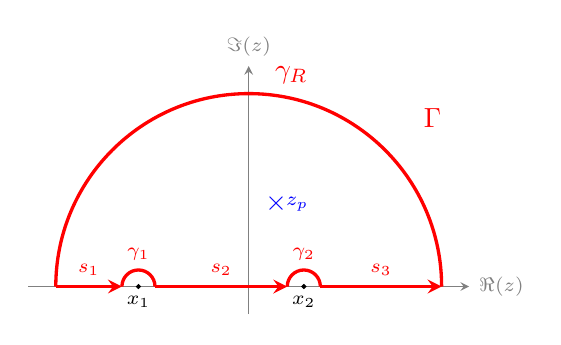
\begin{tikzpicture}[scale=0.7,>=stealth]
    % Ejes
    \draw[->,gray] (-4,0) -- (4,0) node[right] {\scriptsize$\Re(z)$};
    \draw[->,gray] (0,-0.5) -- (0,4) node[above] {\scriptsize$\Im(z)$};

    \node[red, above right] at (3, 2.7) {$\Gamma$};
    % Contorno Grande
    \draw[red,very thick] (3.5,0) arc (0:180:3.5);
    \node[red, above right] at (0.3, 3.5) {$\gamma_R$};

    % Eje real con hendiduras
    % Izquierda a hendidura 1
    \draw[red,very thick, ->] (-3.5, 0) -- (-2.3, 0) node[midway,above] {\scriptsize$s_1$};
    % Hendidura 1 (x1)
    \draw[red,very thick] (-1.7, 0) arc (0:180:0.3);
    \node[below] at (-2,0) {\scriptsize$x_1$};
    \node[red,above] at (-2,0.3) {\scriptsize$\gamma_1$};
    \filldraw (-2,0) circle (1pt);

    % Intermedio
    \draw[red,very thick, ->] (-1.7, 0) -- (0.7, 0) node[midway,above] {\scriptsize$s_2$};

    % Hendidura 2 (x2)
    \draw[red,very thick] (1.3, 0) arc (0:180:0.3);
    \node[below] at (1,0) {\scriptsize$x_2$};
    \node[red,above] at (1,0.3) {\scriptsize$\gamma_2$};
    \filldraw (1,0) circle (1pt);

    % Final
    \draw[red,very thick, ->] (1.3, 0) -- (3.5, 0) node[midway,above] {\scriptsize$s_3$};

    % Polo en el plano superior
    \node[blue] at (0.5, 1.5) {$\times$};
    \node[blue, right] at (0.5, 1.5) {\scriptsize$z_{p}$};

  \end{tikzpicture}
  \caption{Contorno de integración generalizado con hendiduras sobre múltiples polos reales $x_k$.}
  \label{fig:contorno_multiple}
\end{figure}

Consideramos la integral de contorno de $f(z) = Q(z)e^{jmz}$. Por el Teorema de los Residuos, la integral sobre el camino cerrado es igual a $j2\pi$ veces la suma de los residuos encerrados \textit{dentro} del contorno (es decir, solo los polos del semiplano superior, $z_p$):

\begin{equation}
  \oint_\Gamma f(z) dz = j2\pi \sum \res{z=z_p}f(z)
\end{equation}

Desglosando el contorno $\Gamma$, tenemos:
1. La integral sobre el arco grande $\gamma_R$, que tiende a 0 por el Lema de Jordan cuando $R \to \infty$.
2. Las integrales sobre los segmentos $s_1, s_2$ y $s_3$ del eje real, que conforman la integral real impropia.
3. Las integrales sobre las pequeñas semicircunferencias $\gamma_k$ alrededor de cada polo real $x_k$.

Aplicando el límite cuando los radios de las hendiduras tienden a cero ($r \to 0$), y basándonos en la deducción de la sección anterior, cada hendidura aporta:
$$
\lim_{r \to 0} \int_{\gamma_k} f(z) dz = -j\pi \res_{z=x_k}f(z)
$$
El signo negativo surge porque las hendiduras se recorren en sentido horario. Entonces, volviendo al problema inicial, tiene que:
$$
\int_{-\infty}^\infty f(x)dx + \sum_{k=1}^{N} \left( -j\pi \res_{z=x_k}f(z) \right) = j2\pi \sum \res_{z=z_p}f(z)
$$

Despejando la integral real, llegamos a la fórmula generalizada final:

\begin{equation}
\boxed{
  \int_{-\infty}^\infty Q(x)e^{jmx} dx = j2\pi \sum_{\Im(z_p)>0} \res_{z=z_p}f(z) + j\pi \sum_{x_k \in \mathbb{R}} \res_{z=x_k}f(z)
}
\label{eq:formula_general_polos_reales}
\end{equation}

Esta expresión nos dice que para calcular la integral impropia, tomamos los residuos completos de los polos superiores y la \textit{mitad} del residuo de los polos que están justo en la ``frontera'' (el eje real).

\subsection[Racionales analíticas en el eje real]{Racionales analíticas en $\mathbb{R}$}
\label{sec:racionales_analiticas}

Ahora se consideran integrales reales de la forma 
$$
\int_{-\infty}^\infty \frac{p(x)}{q(x)}dx
$$
en donde $p$ y $q$ son polinomios con coeficientes reales y sin factores comunes, $q$ no tiene ceros reales y el grado de $q$ excede el grado de $p$ por al menos 2. Estas condiciones son suficientes para asegurar la convergencia de esta integral impropia.

Como con la clase anterior de integrales, la estrategia es proponer una integral compleja 
$$
\oint_\Gamma \frac{p(z)}{q(z)}dz
$$
tal que podamos encontrar una expresión para la integral real. Para hacer esto primero observe que $q(z)$ tiene coeficientes reales, de manera que sus ceros aparecen en pares complejos conjugados. Suponga que los ceros de $q$ son $z_1,\overline{z_1},z_2,\overline{z_2},\dots,z_m,\overline{z_m}$ con cada $z_j$ en el semiplano superior $\Im(z)>0$ y cada $\overline{z_j}$ en el semiplano inferior $\Im(z)<0$. Sea $\Gamma$ la curva mostrada en la figura \ref{fig:racional_real}, que consiste de la semicircunferencia $\gamma$ y el segmento $S$ en el eje real.
\begin{figure}[ht]
  \centering
  \begin{tikzpicture}[>=stealth]
    \path (-2.5,0) -- (-2,0); % solo para terminar de centrar
    \draw[->,gray] (-2,0) -- (2,0) node[right] {\scriptsize$\Re(z)$};
    \draw[->,gray] (0,-0.2) -- (0,2.2) node[above] {\scriptsize$\Im(z)$};

    \begin{scope}[decoration={
        markings,
        mark=at position 0.1 with {\arrow{>} \node[above right] {$\Gamma$};},
        mark=at position 0.3 with {\arrow{>} \node[above right] {\scriptsize\gamma};},
        mark=at position 0.5 with {\arrow{>}},
        mark=at position 0.7 with {\arrow{>} \node[below right] {\scriptsize$S$};},
        mark=at position 0.9 with {\arrow{>}},
      }]
      \draw[red,very thick,postaction={decorate}] (1.7,0) arc (0:180:1.7) -- cycle;
    \end{scope}
    \node[below] at (1.7,0)  {\scriptsize$R$};
    \node[below] at (-1.7,0) {\scriptsize$-R$};

    \node[blue] at (-1,0.5) {$\times$};
    \node[blue, right] at (-1,0.5) {\scriptsize$z_{m}$};
    \node[blue] at (0.5, 0.7) {$\times$};
    \node[blue, right] at (0.5, 0.7) {\scriptsize$z_{1}$};
  \end{tikzpicture}
  \caption{}
  \label{fig:racional_real}
\end{figure}

Aplicando el Teorema de los Residuos, la integral sobre $\Gamma$ es:
$$
\oint_\Gamma \frac{p(z)}{q(z)}dz = j2\pi \sum_{k=1}^m \res_{z=z_k}\left( \frac{p(z)}{q(z)} \right)
$$
donde la suma se realiza sobre los polos $z_k$ ubicados estrictamente en el semiplano superior ($\Im(z_k) > 0$).
Descomponiendo la integral:
$$
\oint_\Gamma \frac{p(z)}{q(z)}dz = \int_\gamma \frac{p(z)}{q(z)}dz + \int_{-R}^{R} \frac{p(x)}{q(x)}dx
$$
Aquí es crucial la condición sobre los grados de los polinomios. Dado que $\text{grado}(q) \ge \text{grado}(p) + 2$, podemos aplicar la desigualdad ML. Para $|z| = R$ suficientemente grande, $|p(z)/q(z)| \approx k/R^2$. Como la longitud del arco $\gamma$ es $\pi R$, la integral sobre el arco está acotada por $\pi R \cdot (k/R^2) = \pi k / R$, lo cual tiende a cero cuando $R\to\infty$.

Por lo tanto, al tomar el límite $R\to\infty$, la integral sobre $\gamma$ desaparece y obtenemos directamente:
\begin{equation}
  \int_{-\infty}^\infty \frac{p(x)}{q(x)}dx = j2\pi \sum_{\Im(z_k)>0} \res_{z=z_k} \frac{p(z)}{q(z)}
  \label{eq:integral_impropia_racional}
\end{equation}

\begin{example}
  Calcular la siguiente integral usando el método de resolución anterior
  $$
  I = \int_{-\infty}^\infty \frac{1}{x^2+1} dx
  $$
  Identificamos $p(x) = 1$ y $q(x) = x^2+1$.
  Las condiciones se cumplen:
  \begin{itemize}
    \item $q(x)$ no tiene ceros reales.
    \item El grado de $q$ (2) excede al de $p$ (0) en al menos 2.
  \end{itemize}

  Primero, encontramos los polos resolviendo $q(z) = 0$:
  $$
  z^2 + 1 = 0 \implies z = \pm \sqrt{-1} = \pm j
  $$
  Tenemos dos polos simples: $z_1 = j$ y $z_2 = -j$.
  La expresión \eqref{eq:integral_impropia_racional} solo requiere los residuos de los polos en el semiplano superior ($\Im(z) > 0$). En este caso, el único polo relevante es $z_1 = j$.

  Calculamos el residuo de $f(z) = \frac{1}{(z-j)(z+j)}$ en $z=j$:
  $$
  \res_{z=j}f(z) = \lim_{z\to j} (z-j) \frac{1}{(z-j)(z+j)} = \lim_{z\to j} \frac{1}{z+j} = \frac{1}{j+j} = \frac{1}{2j}
  $$

  Finalmente, aplicamos la fórmula:
  \begin{gather*}
  \int_{-\infty}^\infty \frac{1}{x^2+1} dx = j2\pi \sum_{\Im(z_k)>0} \res_{z=z_k}f(z) \\
  I = j2\pi \left( \frac{1}{2j} \right) = \pi
  \end{gather*}

  Este resultado confirma lo que sabemos por cálculo elemental:
  $$
  \int_{-\infty}^\infty \frac{1}{x^2+1} dx = \left. \arctan(x) \right|_{-\infty}^{\infty} = \frac{\pi}{2} - \left(-\frac{\pi}{2}\right) = \pi
  $$
  quedando así resuelta la integral.
\end{example}
